% \begin{savequote}[8cm]
% Alles Gescheite ist schon gedacht worden.\\
% Man muss nur versuchen, es noch einmal zu denken.

% All intelligent thoughts have already been thought;\\
% what is necessary is only to try to think them again.
%   \qauthor{--- Johann Wolfgang von Goethe \cite{von_goethe_wilhelm_1829}}
% \end{savequote}

\chapter{\label{ch:2-draft}Active Phase Separation of Dense Mixtures}

\minitoc

\section{Introduction}

Lipid mixtures can show phase coexistence, even with as little as two phospholipids and a cholesterol component \cite{feigenson_phase_2009}. Model cell membranes, made of these mixtures, result in regions of a liquid ordered and liquid disordered phase,` or a gel phase, depending on the lipid composition. Again, depending on the specific lipid properties the resulting domains can either form macroscopic or nanoscopic domains of each phase. The different phases also exhibit a conformational change in the hydrophobic chains and the neighbouring lipid tails tend to be in the same state. This is a key cooperative effect in causing the phase transition and theoretical descriptions of the equilibrium distributions of the lipids can explain the phase behaviour \cite{wolff_thermodynamic_2011}. In these model systems, the amount of lipid is conserved, however in vivo, local lipid composition actually does change due to membrane recycling and as a result of the activity of enzymes which catalyse lipid synthesis and breakdown.

Theoretical models describing the physics of of liquid-liquid phase separation have developed significantly in recent years, partly driven by the observation of membraneless organelles in vivo \cite{shin_liquid_2017}. A key development in the field has been to add non-equilibrium effects into descriptions of phase transitions including, actively propelled particles \cite{cates_motility-induced_2015}, phoretic transport effects \cite{agudo-canalejo_active_2019} and changes in chemical composition \cite{weber_drops_2021, li_non-equilibrium_2020}. This chapter brings together ideas from non-equilibrium phase transitions and develops a minimal model to describe an active mixture containing an enzyme component.

\section{Equilibrium Phase Separation}

\subsection{Thermodynamics of Fluid Mixtures}

A good example to explore the theory of phase separating mixtures is to study a fluid made up of two components, say, component $A$ and component $B$. To make this mixture, we mix a $N_A$ molecules of component $A$ and $N_B$ molecules of component $B$ to give a mixture of total volume $V = v_A N_A + v_B N_B$, where $v_i$ is the specific volume of the component, the \textit{size} of each molecule. The volume fraction of a component, $\phi_i$, is defined to be $\phi_i = v_i N_i/v$ and for the two component mixture $\phi_A+\phi_B = 1$. To simplify the notation, let $\phi_A=\phi$ and $\phi_B=1-\phi$, and the volume fraction $\phi$ now describes the proportion of the fluid volume that is component $A$. For an incompressible fluid, the total volume is constant and the relevant free energy is the Helmholtz free energy, $F(N_A, N_B, T)$ where $T$ is the temperature of the fluid. The Helmholtz Free energy is an extensive quantity and so the $F(N_A, N_B, T) = V f(\phi, T)$ where $f(\phi, T)$ is the free energy density and this free energy density determines the phase behaviour of the mixture. The mixture will phase separate into two regions with different $\phi$s if this lowers the overall free energy. Labelling the two phases $\mathrm{I}$ and $\mathrm{II}$ the reduced free energy condition is $Vf(\phi, T) = V_{\mathrm{I}} f(\phi_{\mathrm{I}}, T)+ V_{\mathrm{II}} f(\phi_{\mathrm{II}}, T)$ with the total volume being conserved $V = V_{\mathrm{I}}+V_{\mathrm{II}}$. This is equivalent to the free energy density being upper convex, $\frac{\partial^2 f}{\partial \phi^2}$, for some value for $\phi$.

In addition to lowering the free energy of the system, any phase separating regions of a mixture must also be in mechanical and chemical equilibrium, otherwise they would exchange components or volume to reach two equilibrated phases. Chemical equilibrium is achieved when the chemical potential, $\mu$ of each component in each phase is constant and so moving a particle across the phase boundary will not change the free energy, $\mu_i^{\mathrm{I}}=\mu_i^{\mathrm{II}}$. The chemical potential for component $i$ is given by
\begin{equation}
    \mu_i = \left(\frac{\partial F}{\partial N_i}\right)_{V, T} = \left(\frac{\partial f}{\partial \phi_i}\right)_{T}.
    \label{eq:mu_def}
\end{equation}
\todo{Also need to get the volume dependency in here somehow.}
The mechanical equilibrium is achieved when the osmotic pressure, $\Pi$ between the two phases is equal, $\Pi^{\mathrm{I}}=\Pi^{\mathrm{II}}$, where the osmotic pressure is given by \todo{difference between osmotic and mechanical pressure}
\begin{equation}
    \Pi(\phi) = -\left(\frac{\partial F}{\partial V}\right)_{T, N_A} = -f + \phi \left(\frac{\partial f}{\partial \phi}\right)_{T}.
    \label{eq:Pi_def}
\end{equation}
These conditions have a convenient graphical interpretation. The equation for a tangent to the curve $f(\phi)$ at $\phi=\Tilde{\phi}$ can be written as $y=mx+c$. Equation (\ref{eq:mu_def}) and (\ref{eq:Pi_def}) give $y=\mu_A(\Tilde{\phi})\phi - \Pi(\Tilde{\phi})$ and as these thermodynamic quantities must be the same for two coexisting phases, we find that two phases can only coexist if they have a \textit{common tangent}! Figure \ref{fig:phase_sep_scheme} highlights the graphical interpretation of these conditions, where plotting $f(\phi)$ can illuminate the phase behaviour of a mixture. A well mixed homogeneous system prepared with volume fraction $\phi^*$, will therefore be stable as two phase separated with regions volume fraction $\phi_{\mathrm{I}}$ and $\phi_{\mathrm{II}}$ ($\phi_{\mathrm{I}} < \phi_{\mathrm{II}}$) given that $\phi_{\mathrm{I}} < \phi^* < \phi_{\mathrm{II}}$. The conservation of $N_A$ requires $V\phi^* = V_{\mathrm{I}}\phi_{\mathrm{I}} +V_{\mathrm{II}}\phi_{\mathrm{II}}$ and volume conservation gives $V = V_{\mathrm{I}}+V_{\mathrm{II}}$ which determines the volumes of each phase

\begin{equation}
    V_{\mathrm{I}} = \frac{\phi_{\mathrm{II}}-\phi^*}{\phi_{\mathrm{II}}-\phi_{\mathrm{I}}}V
    \quad
    \textrm{and}
    \quad
    V_{\mathrm{II}} = \frac{\phi^*-\phi_{\mathrm{I}}}{\phi_{\mathrm{II}}-\phi_{\mathrm{I}}}V.
\end{equation}

\begin{figure}
    \centering
    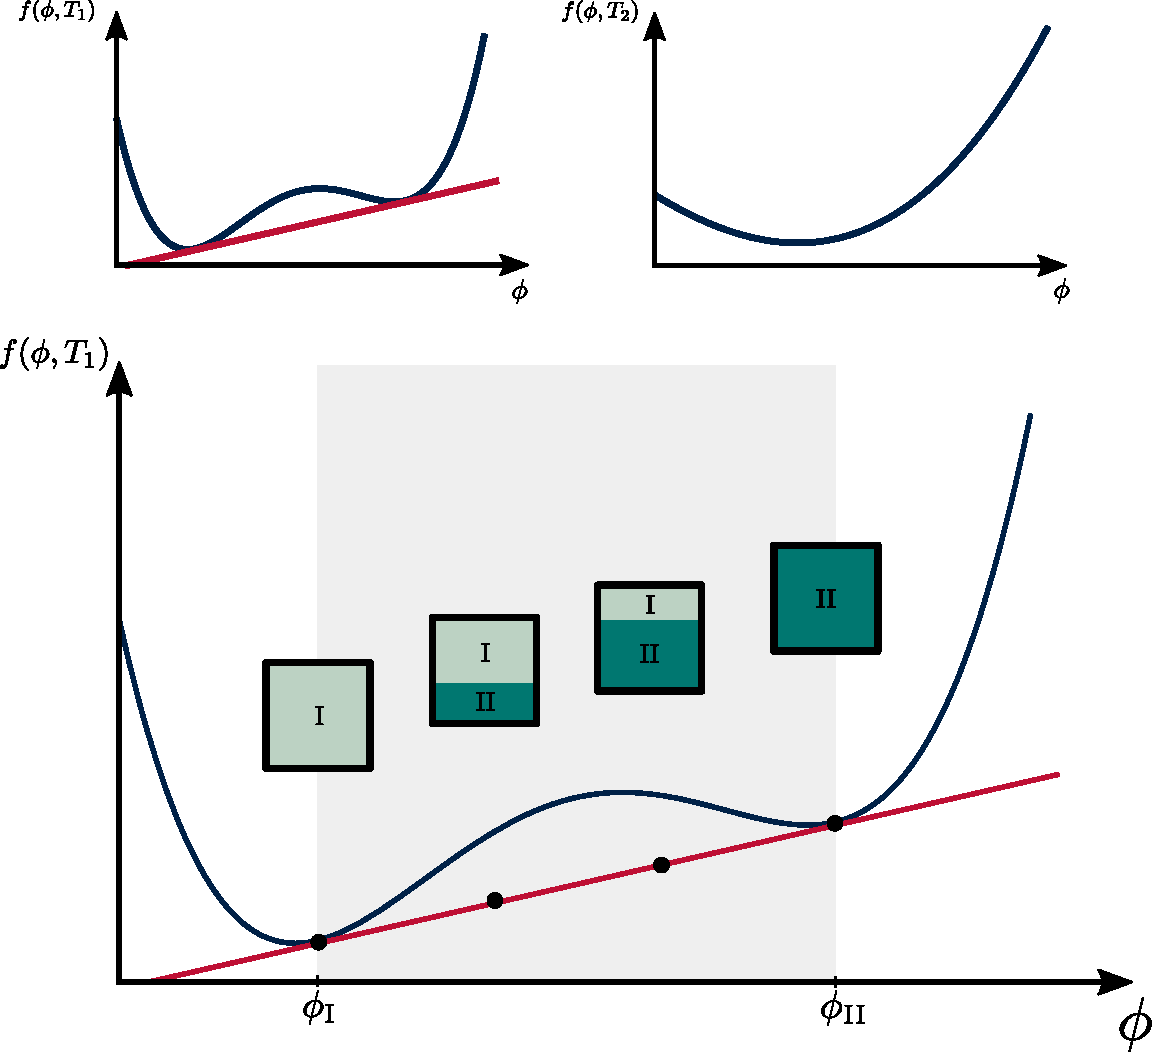
\includegraphics[width=\textwidth]{figures/thermo_solutions.pdf}
    \caption{Caption}
    \label{fig:phase_sep_scheme}
\end{figure}

Often, the shape of the free energy density can be controlled by some external parameter, such as temperature.

\todo{Comment on the energy barrier, spinodal binodal decomposition.}

\subsection{Regular Solution Model}
Mean field models of mixtures can describe the free energy density and predict features of the phase behaviour. The free energy density can be calculated from the Hamiltonian of a system and, again, the $A-B$ binary mixture is a useful place to start. Consider a lattice where each lattice site is occupied by either a molecule of $A$ or a molecule of $B$ where $v_A$ and $v_B$ (the size of each molecule) is the same and additionally define the total number of sites in the lattice $N_{lat} = N_A + N_B$. The different molecules can be configured in many different ways on the lattice however the different configurations will have different energies due to interactions between the molecules. The lattice model can include these interactions by having different contributions to the energy for different pairs of molecules on neighbouring lattice sites. For example, two molecules of $A$ on neighbouring sites will contribute $\epsilon_{AA}$ to the energy of a configuration, two molecules of $B$ contribute $\epsilon_{BB}$ and a molecule of $A$ on a neighbouring lattice site to a molecule of $B$ will contribute $\epsilon_{AB}$. The total energy of a configuration $c$ is then the sum of the interaction energy contribution over all neighbouring lattice sites
\begin{equation}
    E_{c} = N_c^{AA}\epsilon_{AA} + N_c^{AB}\epsilon_{AB} + N_c^{BB}\epsilon_{BB}
\end{equation}
where $N_c^{ij}$ is the number of neighbouring lattice sites, occupied by a molecule of $i$ and molecule of $j$ in the configuration. The free energy desnity can be calculated from the partition function, $Z$, where
\begin{equation}
    f(\phi, T) = -\frac{1}{\beta V}\ln Z
    \label{eq:f_ln}
\end{equation}
\todo{Put a KB T term into the new commands (and define it here)} and the partition function is directly calculated for a canonical ensemble via
\begin{equation}
    Z = \sum_c \exp{-\beta E_c}.
\end{equation}
where the sum is over all configurations. In the thermodynamic limit of large $N_{lat}$ the sum can be well approximated by a mean field approximation. The sum is approximated by replacing the energy of each configuration with the average energy, $\bar{E}$, so the sum now becomes
\begin{equation}
    Z \approx \sum_c \exp(-\beta \bar{E}) = \Omega \exp(-\beta \bar{E})
\end{equation}
where $\Omega$ is the number of unique configurations of molecules on the lattice and is given by
\begin{equation}
    \Omega = \frac{N_{lat}!}{N_A! N_B!}.
\end{equation}

The free energy density in the mean field model is now, with equation (\ref{eq:f_ln}), $f = -\frac{K_B T}{V} (\ln \Omega + \bar{E})$.

The mean energy $\bar{E}$ can be calculated ... The coordination number, $z$, describes the number of nearest neighbours each lattice site, for example $z=4$ in a square lattice. On average $z\phi_i$ of the neighbouring lattice sites will be occupied by a molecule of $i$. For $i \neq j$ the average number of $ij$ neighbour pairs, $\bar{N}^{ij}$, is the number of sites occupied by a molecule of $i$ multiplied by the average the number of neighbouring lattice sites occupied by a molecule of $j$: $\bar{N}^{ij} = N_{lat}\phi_i \times z\phi_j$. When $i=j$ each pair will be double counted (each lattice site occupied by a molecule of $i$ will be considered as both the `main' and `neighbour' site) and so there is an additional factor of 1/2 to prevent double counting. The average energy is therefore
\begin{equation}
\begin{split}
    \bar{E} &= \bar{N}^{AA}\epsilon_{AA} + \bar{N}^
    {AB}\epsilon_{AB} + \bar{N}^{BB}\epsilon_{BB}\\
    &= \frac{1}{2}z N_{lat} \phi^2\epsilon_{AA} + z N_{lat} (1-\phi)\phi\epsilon_{AB} + \frac{1}{2}z N_{lat} (1-\phi)^2 \epsilon_{BB}.
\end{split}
\end{equation}
Using equation (\ref{eq:f_ln}) the free energy density is
\begin{equation}
    f(\phi, T) = -\frac{1}{\beta V}\left(\ln \left(\frac{N_{lat}!}{N_A! N_B!} \right) - \frac{z N_{lat}}{2} \left(\phi^2\epsilon_{AA} + 2(1-\phi)\phi\epsilon_{AB} + (1-\phi)^2 \epsilon_{BB}\right)\right).
\end{equation}
The first term is simplified using Stirling's formula, $\ln N! = N \ln N - N$ for large $N$ to give $\ln\Omega=-N_{lat}(\phi\ln(\phi)+(1-\phi)\ln(1-\phi))$. The average energy term can be simplified as the phase behaviour described in \todo{section reference} was independent of the exact value of $f$, or $\partial f/\partial \phi$ and so the physics of the system is symmetric under a transform $f \rightarrow f + k_1 + k_2\phi$. Specifically, choosing $k_1 = z\epsilon_{BB}/2$ and $k_2 = z(\epsilon_{BB} - \epsilon_{AA})/2$ the free energy now becomes
\begin{equation}
    f(\phi, T) = k_B T (\phi\ln(\phi)+(1-\phi)\ln(1-\phi)) + \chi(1-\phi)\phi
\end{equation}
since $V = N_{lat}$ and define the Flory-Huggins interaction parameter $\chi = -\frac{z}{2 k_B T}(\epsilon_{AA}+\epsilon_{BB}-2\epsilon_{AB})$. \todo{Phase behaviour discussion for chi}

\todo{\begin{enumerate}
    \item Generalise to multi component
    \item Generalise to different volumes
    \item add in interface terms
    \item add in enthalpy terms
\end{enumerate}}
\begin{equation}
    f_{FH} = \sum_{i=1}^{N}\Bigg[\frac{\phi_i}{v_i}\ln\phi_i+\sum_{j=1, j\neq i}^{N}\frac{\chi_{ij}}{2}\phi_i\phi_j + \sum_{j=1}^{N} \frac{K_{ij}}{2}(\nabla\phi_i)\cdot(\nabla\phi_j)\Bigg]
    \label{fh_gen}
\end{equation}

where the scalars $\chi$ and $K$ now become $N \times N$ matrices describing the interactions between components and the surface tensions between domains of different compositions \cite{berry_physical_2018}. The constant number of lattice sites, $N_l$ naturally imposes incompressibility into the model ensuring that $\sum_{i=1}^N\phi_i=1$.
The Flory-Huggins model provides an extension to this regular solution model to reflect the different components as being molecules of different sizes. The model originally described polymers of chain length $N_P$ and introduced a correction to the entropic terms since the monomers on the chain are attached to each other which reduces the number of available configurations. We use this principle generally to extend the regular solution model in equation (\ref{rsm_gen}) to describe components of different size. This gives where $v_i$ describes the relative volumes of the components in the mixture. 

Another important contribution is from the intrinsic energy, the enthalpy, of each type of molecule which will appear proportionally to the number of molecules of that component in the system, $e_i \phi_i / v_i$. Previous work has often ignored this contribution as in a system of constant overall composition this term is simply an additive constant and so does not affect the behaviour of the solution. However the composition of a chemically active system can change and therefore this contribution may affect the system's behaviour.

The phase behaviour of these regular solution models is often dominated by the value of the interaction parameter, $\chi$. For $\chi > 0 $, there is an energetic cost to having different components mixing and can lead to phase separation. The interplay of entropic effects driving a homogeneous mixed state balanced against these additional terms determines the phase transitions. However all of these terms are derived from a free energy and provide an equilibrium description of the system. In fact, additional terms can be added to this equilibrium free energy density, such as terms from a generic external potential or higher order gradient terms. 

\section{Dynamics of Multi-component mixtures}

\subsection{Conserved Dynamics}

\todo{talk about the fact that $\phi$ can vary spatially?}

\subsubsection{Model B Dynamics}
\todo{Physics of active emulsions is quite a good reference for this.}
\todo{Linear response model?}
\todo{Comment on non momentum conservation}
The static lattice picture can describe the free energy of a system, but fails to capture associated dynamics. The lattice model can be extended to include the evolution of a system through configuration space by considering exchange of molecules of neighbouring lattice sites. In this picture (and also physically), the number of molecules of each species does not change and so the behaviour of the volume fraction for each component must obey a continuity equation, namely\cite{li_non-equilibrium_2020}
\begin{equation}
    \dot{\phi}_i = - \nabla \cdot \textbf{J}_i
    \label{eq:continuityModB}
\end{equation}
\todo{keep track of KB Ts} where $i$ labels each component, and $\textbf{J}_i$ is the volume fraction flux. \todo{Tidy the following up. Is Model B phenomenological?} Changes to the distribution of a component will be driven by changes in the free energy and specifically, the associated thermodynamic force, the chemical potential. The canonical Model B dynamics capture this chemical pressure and give the volume fraction flux as
\begin{equation}
    \textbf{J}_i = \sum_j M_{ij}\nabla\mu_j + \textbf{J}^N
    \label{eq:fluxModB}
\end{equation}
where $\mu_i$ is the chemical potential of the $i\th$ component, $M_{ij}$ is a set of generalised mobilities (discussed in the \todo{next section}) and the sum runs over all components in the system. The $\textbf{J}^N$ term describes the noise and must obey the appropriate fluctuation dissipation theorems. In the thermodynamic limit of a noise free model considered here the $ \textbf{J}^N$ contribution vanishes. The chemical potential for each component, $\mu_i$, is given by
\begin{equation}
    \mu_i = v_i\frac{\delta F}{\delta \phi_i}.
\end{equation}
where the additional volume term compared to equation (\ref{eq:mu_def}) is due to the conversion from particle number to volume fraction \todo{clarify this and fit in with the other}.

\subsubsection{Mobilities for Incompressible Models}
\todo{Mazur and de Groot reference?}
The model B dynamics introduce a set of transport coefficients, or mobilities $M_{ij}$, which describe how volume fraction of the $i\th$ component responds to the chemical potential of the $j\th$ component. This is a general form of linear transport relationship found near equilibrium in thermodynamic systems where the flux is proportional $J_i = \sum_{j}L_{ij}\nabla f_{j}$ where the thermodynamic forces are conjugate to the displacements being described. In this generalised description, the transport coefficient matrix described by $L_{ij}$ is both positive semi-definite (positive entropy production rate) and symmetric under exchange of $i, j \rightarrow j, i$. Here however, the flux describes the transport of volume fraction rather than particle number and so the the forces and displacements are not conjugate. As such the reciprocity is broken and $L_{ij} \neq L_{ji}$, however again using the size of individual molecules to convert between volume fraction and number density gives
\begin{equation}
    {M}_{ij} = \frac{v_i}{v_j}{M}_{ji}.
    \label{eq:mobsym}
\end{equation}

The lattice model is incompressible when the total number of lattice sites, $N_{lat}$, is constant. The incompressibility condition can be written as $\sum_i\phi_i = 1$ and so $\sum_i\dot{\phi}_i = 0$. Substituting in the Model B dynamics, equations (\ref{eq:continuityModB}) and (\ref{eq:fluxModB}) give
\begin{equation}
    \sum_i\dot{\phi}_i = \sum_i\;\nabla\cdot\bigg(\sum_j M_{ij}\nabla\mu_j\bigg) = \sum_j\;\nabla\cdot\bigg(\big(\sum_i M_{ij}\big)\nabla\mu_j\bigg) = 0
\end{equation}
In order for this to be true in general, for non-uniform systems, i.e. $\nabla\mu_j \neq 0$, it is necessary for the mobilities to satisfy
\begin{equation}
    \sum_i M_{ij} = 0
    \label{eq:mobinc}
\end{equation}
which constrains the mobilities and enforces the fluid remains incompressible.\cite{kehr_mobility_1989} An $N$-component mixture,  has a total of $N\times N$ mobilities. The reciprocity-like constraint in equation (\ref{eq:mobsym}) reduces the number of free parameters to $N(N+1)/2$ and the incompressibility condition adds a further $N$ constraints to give $N(N-1)/2$ free mobility parameters.

\subsection{Non-Conserved Dynamics}

\subsubsection{Reaction Rates}
In addition to spatial fluxes of component from the Model B dynamics, chemically active mixtures will also permit fluxes in chemical space, i.e. the conversion of a molecule of $i$ to a molecule of $j$. Putting these dynamics into the binary mixture, we allow the reaction $A \rightleftharpoons B$, and an immediate consequence of incompressibility is that the reaction must conserve volume, so here $v_A = v_B$. In general the volume of the reactants must equal the volume of the products which is simple for this 1:1 stoichiometry but could be more complex for non-conserved molecule number. The change in the free energy due to the reaction is $dF = \mu_A dN_A+\mu_B dN_B = (\mu_A - \mu_B)dN_A$ where $dN_A = -dN_B$ by conservation of total molecule number. There is therefore no net conversation between molecules of $A$ and $B$ when $\mu_A = \mu_B$ and \todo{justify/explain this} the rate of the reaction is given by... Considering detailed balance for the system constrains the relationship between the forward and backward reaction rates
\begin{equation}
    \frac{r_{A \rightarrow B}}{r_{B \rightarrow A}} = \exp\Bigg(\frac{\mu_A - \mu_B}{k_B T}\Bigg)
    \label{db_constr}
\end{equation}
which allows us to identify the net transfer from $A \rightarrow B$ as
\begin{equation}
    r_{A \rightarrow B} - r_{B \rightarrow A} = K\Bigg(\exp\bigg(\frac{\mu_A - \mu_B}{k_B T}\bigg)-1\Bigg)
    \label{eq:sponrate}
\end{equation}
which makes sense as if $\mu_A > \mu_B$ then we have net $A \rightarrow B$, when $\mu_B > \mu_A$ then we have net $B \rightarrow A$ and at equilibrium $\mu_A = \mu_B$\cite{weber2019physics}.
\todo{Example of how this reduces to mas action}

\subsubsection{Enzymatic Activity}
Enzymes act as catalysts in biological reactions and increase the rate of a reaction. This can be achieved by the presence of an active site that allows the reaction to occur or via some alternative reaction route    fuel driven reaction that occurs only in the presence of this \textit{enzyme} component. The reaction that now occurs is
\begin{equation}
    \text{Enzyme + Fuel} + A \leftrightharpoons \text{Enzyme + Waste} + B
\end{equation}
where the system is in contact with a Fuel and Waste reservoir that maintains constant chemical potentials, $\mu_{Fuel}$ and $\mu_{Waste}$ and define $\Delta\mu \equiv \mu_{Fuel}-\mu_{Waste}$ which is also constant. Alternatively, $\Delta \mu$ could represent the energy transferred by a photon in a light-activated catalytic reaction. Using equation (\ref{db_constr}) the rate of $A \rightarrow B$ of this reaction in the presence of the enzyme can be written as
\begin{equation}
    r_{A \rightarrow B,E} - r_{B \rightarrow A,E} = K'\rho_\textrm{E}\Bigg(\exp\bigg(\frac{\mu_A - \mu_B + \Delta\mu}{k_B T}\bigg)-1\Bigg)
    \label{eq:enzrate}
\end{equation}
where the reaction rate is proportional to the local concentration of the enzyme component, $\rho_\textrm{E}$ and $K'$ is the modified rate constant. Reaction kinetics of enzymes are often described using Michaelis–Menten kinetics where $r_{A\rightarrow B}\sim\rho_\textrm{E}\rho_\textrm{A}/(K_{M}+\rho_\textrm{A})$ where $K_M$ is the Michaelis constant and $\rho_\textrm{A}$ is the concentration of the substrate, A\cite{murray_mathematical_1993}. In both  descriptions of the kinetics, the rate increases linearly with $\rho_\textrm{E}$ however, equation (\ref{eq:enzrate}) will additionally capture the effect of interactions on the rate of conversion when compared to the Michalis-Menten rate.

\section{Minimal Model of an Active Mixture}

The simplest model that will encapsulate all of these effects requires at least two components for a chemical reaction to occur, e.g. $S \rightleftharpoons P$ (substrate to product) and a third enzyme component (E), that permits the driven, catalytic reaction described in equation (\ref{eq:enz_rates}). At every point in space and time system is parameterised by three volume fractions; $\phis(\bm{r},t)$, $\phip(\bm{r},t)$ and $\phie(\bm{r},t)$, corresponding to individual molecules of volume $\vs$, $\vp$ and $\ve$ respectively. The mixture is incompressible and so $\phis+\phip+\phie=1$ everywhere and consequently the reaction requires, $\vs = \vp$. In living systems, enzymes have much more complex structures than reactants and so we expect the size of this component to be much larger $\ve > \vs, \vp$\cite{berg_biochemistry_2002}. This increased size is also expected to result in increased viscous drag and reduced mobility for an enzyme compared to the other components. The Flory-Huggins theory of suspensions gives the free energy of the system as $F = \int \mathrm{d}\bm{r} f_\mathrm{FH}$, with the free energy density
\begin{equation}
    f_\mathrm{FH}(\{\phi_i\}) = \sum_{i=1}^{N} \frac{1}{v_i} \big[\varepsilon_i\phi_i + k_\mathrm{B}T \phi_i \big(\log\phi_i-1\big) \big], 
    \label{eq:fh_gen}
\end{equation}
where $\varepsilon_i$ is the enthalpy of component $i$. Importantly, we do not include any interaction terms in the free energy, in particular $f_\mathrm{FH}$ does not contain terms of the usual form $\chi_{ij}\phi_i \phi_j$. This implies that phase separation in this system would be impossible at equilibrium. The chemical potential of a component is given by
\begin{equation}
    \mu_i = e_i + \log\phi_i + 1 \quad \text{and so} \quad \nabla\mu_i = \frac{1}{\phi_i}\nabla\phi_i
    \label{eq:chempot}
\end{equation}
which drive the conserved dynamics of Model B. For the mobilities we assume the common form where $M_{ij} = -\beta D_{ij}\phi_i\phi_j$ for $i \neq j$ and $\beta \equiv (k_\mathrm{B}T)^{-1}$. The mobility constraints imply $M_{jj}= - \sum_{i\neq j} M_{ij}$ and $v_j D_{ij} = v_i D_{ji}$ \cite{KRAMER1984473, kehr_mobility_1989, mao_designing_2020, bo_stochastic_2021}. The transport coefficients $D_{ij}$ determine the rate at which the components respond to local effective concentration gradients and exchange positions, and as such are inherently related to the phenomena of diffusiophoresis, cross-diffusion and Maxwell-Stefan diffusion \cite{suppmat}.

We make the model active by allowing non-equilibrium (fuelled) conversion between two components, substrate (S) and product (P), catalyzed by an enzyme (E). This can be described by the reaction E+S+F $\rightleftharpoons$ E+P+W, where F and W represent fuel and waste molecules, respectively. We do not model the dynamics of the fuel and waste here, but assume that the system is in contact with a reservoir that maintains constant chemical potentials, $\muf$ and $\muw$, and define $\Delta\mu \equiv \muf-\muw$. The catalysed reaction converts substrate to product with rate $\rcat$ and we also model the spontaneous reaction (does not require enzyme) which converts substrate to product at rate $\rspo$ (note that these contributions might be negative as this flux is always expressed in the direction $S \rightarrow P$). Evaluating equations (\ref{eq:sponrate}) and (\ref{eq:enzrate}) with the chemical potential from equation (\ref{eq:chempot}) gives
\begin{align}
    \rspo &= \rspo^{\mathrm{S}\to\mathrm{P}} - \rspo^{\mathrm{P}\to\mathrm{S}} = \kspo[e^{\beta \Delta \varepsilon}\phis - \phip],\\
    \rcat &= \rcat^{\mathrm{S}\to\mathrm{P}} - \rcat^{\mathrm{P}\to\mathrm{S}} = \kcat\phie[\phis-\phip e^{-\beta(\Delta \varepsilon+ \Delta\mu)}],
    \label{r_cat}
\end{align}
where $\Delta e = e_S - e_P$. The rate constants here have been scaled to better disentangle the effects of the various parameters; $k_{spo} = K_{spo}/\phi_P$ and $k_{cat} = K_{cat}e^{-(\Delta e + \Delta \mu)}/(\ve \phi_P)$. We will typically take $\Delta \varepsilon<0$ and $\Delta \varepsilon + \Delta \mu>0$, so that the spontaneous and catalyzed reactions run preferentially in the P$\to$S and S$\to$P directions, respectively; see Fig.~\ref{fig:cartoon-schematic}.

Combining the conserved and non-conserved dynamics and defining $R\equiv\rspo+\rcat$ results in the evolution equations for the three-component system
\begin{align}
    \dot{\phie} &= \bm{\nabla} \cdot \big(\Mee\bm{\nabla}\mue + \Mes\bm{\nabla}\mus + \Mep\bm{\nabla}\mup\big), \label{eq:evoE}\\
    \dot{\phis} &= \bm{\nabla} \cdot \big(\Mse\bm{\nabla}\mue + \Mss\bm{\nabla}\mus + \Msp\bm{\nabla}\mup\big) - R, \label{eq:evoS}\\
    \dot{\phip} &= \bm{\nabla} \cdot \big(\Mpe\bm{\nabla}\mue + \Mps\bm{\nabla}\mus + \Mpp\bm{\nabla}\mup\big) + R. \label{eq:evoP}
\end{align}

\section{Catalysis Induced Phase Separation}
\subsection{Stability of the Homogeneous Steady State}
The minimal model in equations (\ref{eq:evoE})--(\ref{eq:evoP}) have a homogeneous steady-state solution when $R=0$. Since the enzyme component is conserved in the system we can define $\phie^*$ as the average enzyme volume fraction in the initialisation of a system, such that the total volume of enzyme component in the system is $V \times \phie^*$. For any $\phie^*$, solving $R=0$ gives steady state volume fraction for the substrate and product components
\begin{align}
    \phis^* &= \phisp^*\frac{\kspo + \kcat\phie^*e^{-\beta(\Delta \varepsilon + \Delta\mu)}}{\kspo + \kcat\phie^*e^{-\beta (\Delta \varepsilon + \Delta\mu)}+\kspo e^{\beta \Delta \varepsilon} + \kcat\phie^*}
    \label{sstar}
    \\
    \phip^* &= \phisp^*\frac{\kspo e^{\beta \Delta \varepsilon} + \kcat\phie^*}{\kspo + \kcat\phie^*e^{-\beta (\Delta \varepsilon + \Delta\mu)}+\kspo e^{\beta \Delta \varepsilon} + \kcat\phie^*}
    \label{pstar}
\end{align}
with $\phisp^*=1-\phie^*$, which is the average volume fraction of the substrate and product combined $(\phisp^*=\phis^*+\phip^*)$ and is also conserved.

\todo{start of supmat}

We can study the linear stability of this homogeneous steady-state by considering a small perturbation $\phi_i(\bm{r},t) = \phi_i^* + \delta\phi_i(\bm{r}, t)$, giving $\mu_i(\bm{r},t) = \mu_i^* + \delta\mu_i(\bm{r},t)$ and define mobilities at the homogeneous steady state $M^*_{ij} = M_{ij}(\phie^*, \phis^*, \phip^*)$. To first order in the perturbation $\delta\mu(\bm{r},t) = \frac{\delta\phi_i(\bm{r},t)}{\phi_i^*}$ and thus $\bm{\nabla}\mu_i(\bm{r},t) = \frac{1}{\phi_i^*}\bm{\nabla}\delta\phi_i(\bm{r},t)$. Additionally, define how the reaction rate changes under a small change in $\phi_i$ to be $R_i$, such that $R = \Rs \delta \phis - \Rp \delta \phip + \Ree \delta \phie$ where the sign changes for the product component to keep $\Rp > 0$. This gives
\begin{align}
    \Rs &\equiv \kspo e^{\beta \Delta \varepsilon} + \kcat\phie^* \\
    \Rp &\equiv \kspo + \kcat\phie^*e^{-\beta (\Delta \varepsilon+\Delta \mu)} \\
    \Ree &\equiv k_\mathrm{cat} [ \phis^* - \phip^* e^{-\beta (\Delta \varepsilon + \Delta \mu)}] = \phi^*_\mathrm{s+p} \frac{k_\mathrm{cat} k_\mathrm{spo} (1-e^{-\beta \Delta \mu})}{k_\mathrm{spo} + k_\mathrm{cat} \phie^* e^{-\beta (\Delta \varepsilon + \Delta \mu)} + k_\mathrm{spo} e^{\beta \Delta \varepsilon} + k_\mathrm{cat} \phie^* }.
\end{align}
The governing equations for the perturbations $\delta\phi_i (\bm{q},t) $ in Fourier space are found as follows\\
\noindent
\makebox[\textwidth]{\parbox{1.3\textwidth}{%
\begin{equation}
\begin{pmatrix}
\dot{\delta\phie}\\
\dot{\delta\phis}\\
\dot{\delta\phip}\\
\end{pmatrix} =
\underbrace{
\begin{pmatrix}
(\Mse^*+\Mpe^*)\frac{\bm{q}^2}{\phie^*} & -\Mse^*\frac{\ve}{\vs}\frac{\bm{q}^2}{\phis^*} & -\Mpe^*\frac{\ve}{\vs}\frac{\bm{q}^2}{\phip^*}\\
-\Mse^*\frac{\bm{q}^2}{\phie^*} - \Ree  & \big(\Msp^* + \Mse^*\frac{\ve}{\vs}\big)\frac{\bm{q}^2}{\phis^*} - \Rs  & -\Msp^*\frac{\bm{q}^2}{\phip^*} + \Rp \\
-\Mpe^*\frac{\bm{q}^2}{\phie^*}  + \Ree  & -\Msp^*\frac{\bm{q}^2}{\phis^*} + \Rs  & \big(\Mpe^*\frac{\ve}{\vs}+\Msp^*\big)\frac{\bm{q}^2}{\phip^*} - \Rp \\
\end{pmatrix}
}_{\cal C}
\begin{pmatrix}
\delta\phie\\
\delta\phis\\
\delta\phip\\
\end{pmatrix}.
\end{equation}}}
In this formulation, we can explicitly see the incompressibility being imposed as the columns of $\cal C$ sum to zero.
We now eliminate one of the components, e.g. $\delta\phip = -\delta\phie - \delta\phis$, and define a $2\times2$ matrix, $\cal K$, describing the evolution of the remaining components. This is obtained from $\cal C$ by subtracting the last column from the other two (i.e. ${\cal K}_{ij} = {\cal C}_{ij} - {\cal C}_{i3}$ for $i, j \in {1, 2}$), giving
\newline
\noindent
\makebox[\textwidth]{\parbox{1.3\textwidth}{%
\begin{equation}
\begin{pmatrix}
\dot{\delta\phie}\\
\dot{\delta\phis}\\
\end{pmatrix} =
\underbrace{
\begin{pmatrix}
(\Mse^*+\Mpe^*)\frac{\bm{q}^2}{\phie^*} +\Mpe^*\frac{\ve}{\vs}\frac{\bm{q}^2}{\phip^*}& -\Mse^*\frac{\ve}{\vs}\frac{\bm{q}^2}{\phis^*} + \Mpe^*\frac{\ve}{\vs}\frac{\bm{q}^2}{\phip^*}\\
-\Mse^*\frac{\bm{q}^2}{\phie^*} - \Ree  + \Msp^*\frac{\bm{q}^2}{\phip^*} - \Rp  & \big(\Msp^* + \Mse^*\frac{\ve}{\vs}\big)\frac{\bm{q}^2}{\phis^*} - \Rs  + \Msp^*\frac{\bm{q}^2}{\phip^*} - \Rp \\
\end{pmatrix}
}_{\cal K}
\begin{pmatrix}
\delta\phie\\
\delta\phis\\
\end{pmatrix}.
\end{equation}}}
The eigenvalues of ${\cal K}$ determine the stability of the steady state. The system is stable if and only if all eigenvalues of ${\cal K}$ are negative. The Onsager relations and the non-negativity of $R_i$ mean ${\cal K}_{1,1}$ and ${\cal K}_{2,2}$ are always negative, so $\text{tr}({\cal K}) < 0$ and there is therefore one positive eigenvalue if $\det({\cal K})<0$. The instability condition then becomes
\begin{equation}
\begin{split}
    \Bigg((\Mse^*+\Mpe^*)&\frac{\bm{q}^2}{\phie^*} + \Mpe^*\frac{\ve}{\vs}\frac{\bm{q}^2}{\phip^*}\Bigg)\Bigg(\big(\Msp^* + \Mse^*\frac{\ve}{\vs}\big)\frac{\bm{q}^2}{\phis^*} - \Rs  + \Msp^*\frac{\bm{q}^2}{\phip^*} - \Rp \Bigg) \\
    &< \Bigg(-\Mse^*\frac{\ve}{\vs}\frac{\bm{q}^2}{\phis^*} + \Mpe^*\frac{\ve}{\vs}\frac{\bm{q}^2}{\phip^*}\Bigg)\Bigg(-\Mse^*\frac{\bm{q}^2}{\phie^*} - \Ree  + \Msp^*\frac{\bm{q}^2}{\phip^*} - \Rp \Bigg).
\end{split}
\label{hi_ord_ins}
\end{equation}
When $\bm{q}$ is very large, we expect the system to be stable as in this regime the evolution is dominated by diffusive relaxation. For $\bm{q} = 0$, the system is at critical stability due to global conservation, as this corresponds to a uniform change in $\phi_i$. As such, since this condition only depends on $\bm{q}^2$ and $\bm{q}^4$, the instability is satisfied if and only if it is satisfied for very small $\bm{q}^2$. With this in mind we take Eq. (\ref{hi_ord_ins}) to order $\sim\bm{q}^2$ which gives
\begin{align}
    \frac{1}{\ve\phie^*}+\frac{1}{\vs(1-\phie^*)} < \frac{\Ree }{\vs(1-\phie^*)}\bigg(\frac{\gamma_\mathrm{p}}{\Rs }-\frac{\gamma_\mathrm{s}}{\Rp }\bigg)
    \label{eq_form_cond}
\end{align}
where we have defined
\begin{equation}
    \gamma_\mathrm{s} \equiv \frac{\Mse^*}{\Mse^*+\Mpe^*} \quad \text{   and    } \quad \gamma_\mathrm{p} \equiv \frac{\Mpe^*}{\Mse^*+\Mpe^*}.
\end{equation}
This condition can also be written to constrain the relative volumes in the system
\begin{equation}
    \frac{\vs}{\ve} < \frac{\phie^*}{1-\phie^*}\Bigg[\Ree \bigg(\frac{\gamma_\mathrm{p}}{\Rs }-\frac{\gamma_\mathrm{s}}{\Rp }\bigg) - 1\Bigg],
    \label{vol_ins}
\end{equation}
which shows that the instability is favoured by larger enzymes, the biologically relevant case. With the common choice of mobilities ($\Mes = -\beta \Dse\phie\phis$ and $\Mpe = -\beta \Dpe\phie\phip$) the instability becomes
\begin{equation}
    \frac{1}{\ve\phie^*}+\frac{1}{\vs(1-\phie^*)} < \frac{\Ree }{\vs(1-\phie^*)}\frac{\Dpe-\Dse}{\Dpe\Rs +\Dse\Rp }. \label{eq:inst}
\end{equation}
In calculating this condition, we eliminated the product component from the system and determined the stability by considering the other two components. Eliminating either of the other components gives the same result.

Since the left hand side of (\ref{eq:inst}) is always positive, an instability is possible only if the right hand side is positive as well. The sign of the right hand side is controlled by that of $(1-e^{-\beta\Delta \mu})(\Dpe-\Dse)$, which has several implications. First, an equilibrium system with $\Delta\mu=0$ is always stable, as expected from equilibrium theory of a multicomponent mixture with no interactions. Second, for a catalytic reaction favouring product formation with $\Delta \mu>0$, an instability is possible only if $\Dpe>\Dse$. Third, if $\Dpe=\Dse$ the system is always stable. Intuitively, the instability arises from an enzyme rich region locally producing a higher concentration of product ($\Delta \mu > 0$) and creating a gradient of the product concentration. Due to the unequal response of the enzyme to gradients of substrate and product when $\Dpe>\Dse$, the enzyme will preferentiall move up the product gradient towards the enzyme rich region, resulting in effective enzyme-enzyme attractive interactions and further aggregation. Figure \todo{fig} summarises this mechanism.

\subsection{Numerical Simulation}

Numerical solution of the evolution equations (\ref{eq:evoE})--(\ref{eq:evoP}) confirms the existence of this instability. We initialize a 1D system
with small number-conserving random variations around $\phi_i^*$. When the system is unstable, regions of high and low enzyme concentrations develop spontaneously [see Fig.~\ref{fig:bino_spino}(c)] and coarsen over time, ultimately resulting in two distinct phase-separated domains. Moreover, varying the amount of enzyme in the system only changes the relative size of the high and low concentration domains, without affecting the concentration values in the two domains, which suggests the existence of a binodal line, as in equilibrium phase separation. We observed this behavior for all parameters which we simulated ($\kcat/\kspo\approx 1 \text{--} 100$, $\ve/\vs\approx 2 \text{--} 100$, $-\Delta \varepsilon\approx 5 \text{--} 30 k_{\rm B} T$, $\Delta \mu\approx5 \text{--} 50k_{\rm B} T$,  $\Dpe/\Dse\approx1 \text{--} 100$). The observation of macroscopic phase separation, rather than pattern formation or microphase separation, is further supported by the linear stability analysis showing an instability at the largest wavelengths ($q^2 \to 0$), rather than at finite wavelengths. We also note that studies of two-component mass-conserving reaction-diffusion systems, which have significant parallels to the model studied here \cite{suppmat}, have shown that these systems exhibit uninterrupted coarsening leading to macrophase separation at long times \cite{brauns2020phase,brauns2021wavelength}.

\begin{figure}
    \centering
    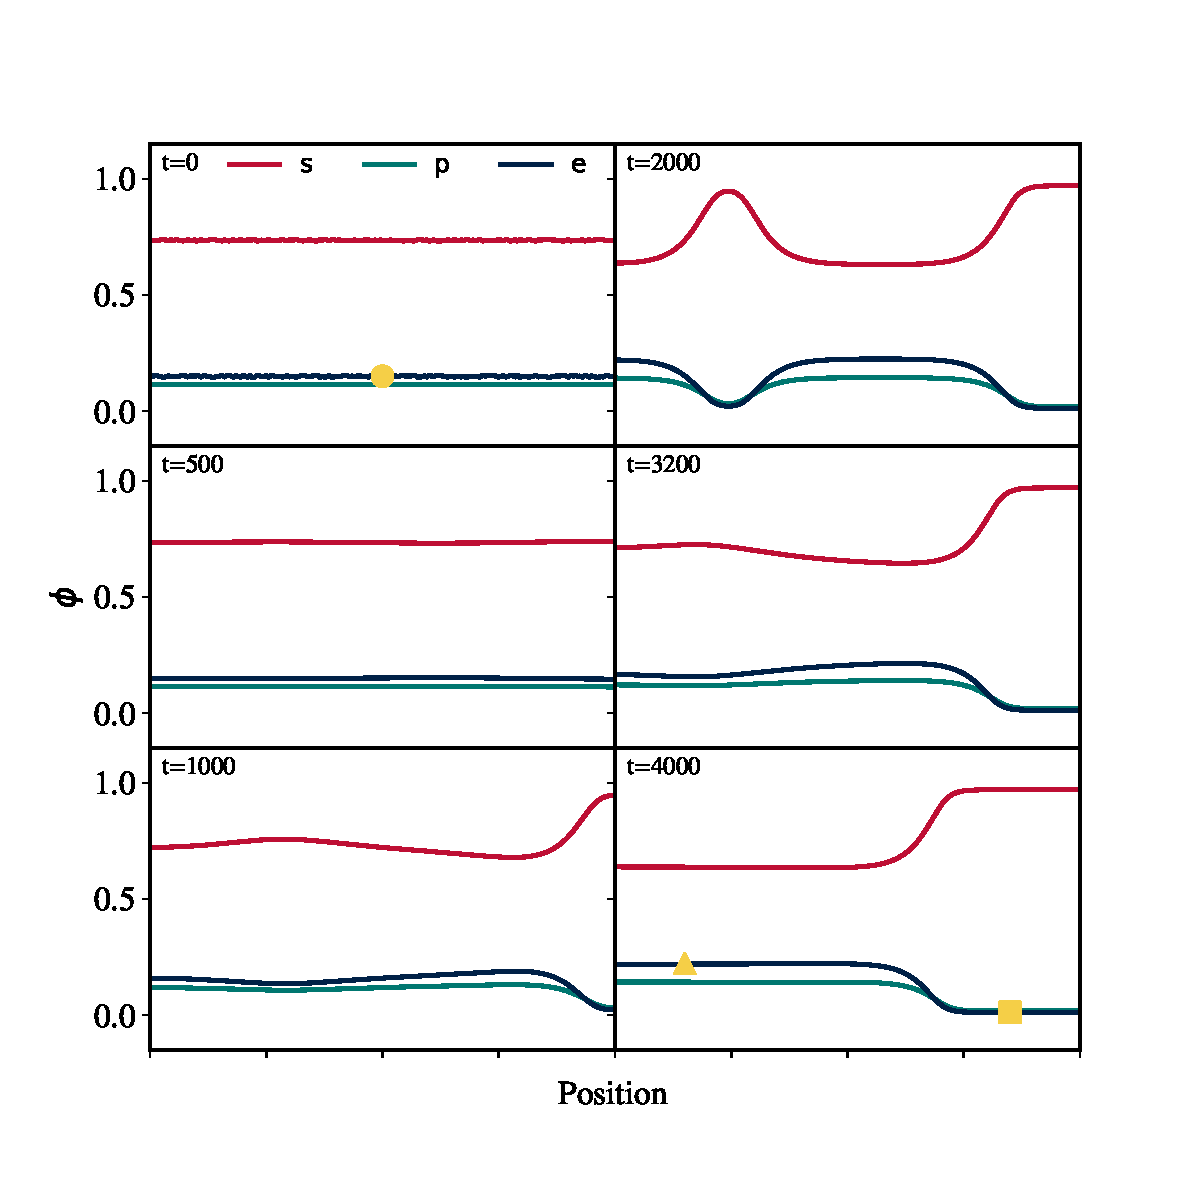
\includegraphics[width=\textwidth]{figures/CIPSnumeric.pdf}
    \caption{Caption}
    \label{fig:phase_sep_scheme}
\end{figure}

A quick check for eliminating the substrate instead can be seen by noticing the expression is invariant under $S, P \rightarrow P, S$ and $R_E \rightarrow -R_E$, which is the same difference between the second and third rows of $C'$. Prior work often imposes incompressibility by eliminating one of the components and using $\phi_i = 1-\sum_{j,j\neqi}\phi_j$. This can be useful when eliminating a solvent component, but in dense systems such as this three component mixture all components need to be kept on an equal footing to see the coupling between responses to gradients as a consequence of the incompressibility.

\subsection{Stability of a four-component system}

An additional solvent component (e.g. cholesterol in a lipid mixture) can be added to the system similarly to the enzyme component, with conserved dynamics and no reaction terms. Following a similar procedure as for the no-solvent case, we can expand around a steady state where we now have $\phisp^* \neq 1 - \phi^*_\mathrm{E}$ but $\phiw^* = 1 - \phisp^* - \phi^*_\mathrm{E}$. We can eliminate the solvent volume fraction to give a $3\times3$ matrix describing the evolution of E, S, and P volume fractions
\begin{equation}
    (\dot{\delta\phie}, \dot{\delta\phis}, \dot{\delta\phip})^T = {\cal K}_{\rm w}(\delta\phie, \delta\phis, \delta\phip)^T    
\end{equation}
with
\newline
\noindent
\makebox[\textwidth]{\parbox{1.3\textwidth}{%
\begin{equation}
   {\cal K}_{\rm w} = 
\begin{tiny}
\begin{pmatrix}
(\Mse^*+\Mpe^*+\Mwe^*)\frac{\bm{q}^2}{\phie^*}+\Mwe^*\frac{\ve}{\vw}\frac{\bm{q}^2}{\phiw^*} & -\Mse^*\frac{\ve}{\vs}\frac{\bm{q}^2}{\phis^*}+\Mwe^*\frac{\ve}{\vw}\frac{\bm{q}^2}{\phiw^*} & -\Mpe^*\frac{\ve}{\vs}\frac{\bm{q}^2}{\phip^*}+\Mwe^*\frac{\ve}{\vw}\frac{\bm{q}^2}{\phiw^*}\\
-\Mse^*\frac{\bm{q}^2}{\phie^*}-\Ree +\Mws^*\frac{\vs}{\vw}\frac{\bm{q}^2}{\phiw^*} & (\Mse^*\frac{\ve}{\vs}+\Msp^*+\Mws^*)\frac{\bm{q}^2}{\phis^*}-\Rs  +\Mws^*\frac{\vs}{\vw}\frac{\bm{q}^2}{\phiw^*}& -\Msp^*\frac{\bm{q}^2}{\phip^*}+\Rp +\Mws^*\frac{\vs}{\vw}\frac{\bm{q}^2}{\phiw^*}\\
-\Mpe^*\frac{\bm{q}^2}{\phie^*}+\Ree +\Mwp^*\frac{\vs}{\vw}\frac{\bm{q}^2}{\phiw^*} & -\Msp^*\frac{\bm{q}^2}{\phis^*}+\Rs +\Mwp^*\frac{\vs}{\vw}\frac{\bm{q}^2}{\phiw^*} & (\Mpe^*\frac{\ve}{\vs}+\Msp^*+\Mwp^*)\frac{\bm{q}^2}{\phip^*}-\Rp +\Mwp^*\frac{\vs}{\vw}\frac{\bm{q}^2}{\phiw^*}\\
\end{pmatrix}
\end{tiny}
\end{equation}
}}

We now assume that the substrate and product dynamics are fast in comparison to the enzyme. Setting $\dot{\delta\phis}=\dot{\delta\phip}=0$ gives
\begin{equation}
    \dot{\delta\phie} = ({\cal K}_{\rm w}^{-1})_{1, 1}\delta\phie
\end{equation}
and so the system is unstable when
\begin{equation}
    ({\cal K}_{\rm w}^{-1})_{1, 1} = \frac{({\cal K}_{\rm w})_{2, 2}({\cal K}_{\rm w})_{3, 3}-({\cal K}_{\rm w})_{2, 3}({\cal K}_{\rm w})_{3, 2}}{\det({\cal K}_{\rm w})} \geq 0.
    \label{solvstab}
\end{equation}
The numerator of (\ref{solvstab}) is, to order $\bm{q}^2$,
\begin{equation}
    \bm{q}^2\Bigg[-\Rp \frac{\Mse^*\frac{\ve}{\vs}+\Mws^*}{\phis^*}-\Rs \frac{\Mpe^*\frac{\ve}{\vs}+\Mwp^*}{\phip^*}-\frac{\vs}{\vw\phiw^*}\big(\Rs +\Rp \big)\big(\Mws^*+\Mwp^*\big)\Bigg].
    \label{solvnum}
\end{equation}
With the common choice of mobilities, $M_{ij}<0$ for $i \neq j$, and $R_i \geq 0$, the expression (\ref{solvnum}) is positive and the instability condition is simply
\begin{equation}
    \det({\cal K}_{\rm w}) > 0,
\end{equation}
which marks the transition from having all negative eigenvalues to having two negative and one positive eigenvalue. This expression is used to derive the instability (spinodal) line in Fig.~2(d) of the main text.

The determinant of ${\cal{K}}_{\rm w}$ has many terms and even when truncated to order $\bm{q}^2$ it is not a manageable expression. A key observation is that in the low solvent limit ($\phiw \to 0$), and assuming Kramer's form for the mobilities, we recover the no-solvent case, as can be seen in \todo{Fig.~2(d)}.

\subsection{Effective free energy and binodal}

In the macroscopic limit, we expect the substrate-product equilibrium in the bulk of each phase to be governed by the reaction terms that act locally, rather than by spatial diffusion. This implies that the substrate and product concentrations are enslaved to the enzyme concentration by $\phis \approx \phis^*(\phie)$ and $\phip \approx \phip^*(\phie)$, with the functions defined in (\ref{sstar}) and (\ref{pstar}). The system and its dynamics can now be described entirely as a function of the enzyme volume fraction $\phie$. All volume fractions, chemical potentials and mobilities describing the system are enslaved to $\phie$. As such equation (\ref{eq:evoE}) now becomes
\begin{equation}
    \dot{\phie} = \bm{\nabla} \cdot \left(\left(\Mee\frac{\mathrm{d}\mue}{\mathrm{d}\phie} + \Mes\frac{\mathrm{d}\mus}{\mathrm{d}\phie} + \Mep\frac{\mathrm{d}\mup}{\mathrm{d}\phie}\right)\bm{\nabla}\phie\right)
\end{equation}
We can recast the dynamics of the enzyme as $\dot{\phie}\approx \bm{\nabla} \cdot (\Mee\bm{\nabla}\mu_\mathrm{eff})$ with an effective chemical potential for the enzyme that satisfies
\begin{equation}
    \bm{\nabla}\mu_\mathrm{eff} = \left(\frac{\text{d}\mue}{\text{d}\phie} + \frac{\Mes}{\Mee}\frac{\text{d}\mus}{\text{d}\phie} + \frac{\Mep}{\Mee}\frac{\text{d}\mup}{\text{d}\phie}\right)\bm{\nabla}\phie.
\end{equation}
This means that by direct integration of the term in brackets with respect to $\phie$ we can calculate an effective chemical potential for the limit of fast reactions in the system. For the minimal model used here this integral can be evaluated exactly to give
\begin{equation}
    \frac{\mu_\mathrm{eff}(\phie)}{k_{\rm B} T} =  \log \phie - \frac{\ve}{\vs} \log[\Dse \phis^* (\phie) + \Dpe \phip^*(\phie)].
\end{equation}
We can also identify an effective free energy density $f_\mathrm{eff}(\phie)$, such that $\mu_\mathrm{eff}=\ve\frac{\mathrm{d} f_\mathrm{eff}}{\mathrm{d} \phie}$, which can be explicitly calculated by direct integration to give
\begin{equation}
\begin{split}
    \frac{f_\mathrm{eff}(\phie)}{k_{\rm B} T} &= \frac{1}{\vp}\frac{\kspo}{\kcat}\Bigg(\frac{1+e^{\beta \Delta \varepsilon}}{1+e^{-\beta (\Delta \varepsilon + \Delta \mu)}}\log\left[\frac{\kcat}{\kspo}\phie + e^{\beta (\Delta \varepsilon + \Delta \mu)}(1+e^{\beta \Delta \varepsilon} + \frac{\kcat}{\kspo}\phie)\right] \\
    -& \frac{\Dse+\Dpe e^{\beta \Delta \varepsilon}}{\Dpe+\Dse e^{-\beta (\Delta \varepsilon + \Delta \mu)}}\log\Big[\Dse\frac{\kcat}{\kspo}\phie + e^{\beta (\Delta \varepsilon + \Delta \mu)}(\Dse+\Dpe e^{\beta \Delta \varepsilon} + \Dpe \frac{\kcat}{\kspo}\phie)\Big]\Bigg) \\
    +&\left(\frac{1}{\vp}-\frac{1}{\ve}\right)\phie + \frac{1}{\vp}\log[1-\phie] + \phie\bigg(\frac{1}{\ve}\log\phie - \frac{1}{\vp} \log[\Dse\phis^*(\phie)+\Dpe\phip^*(\phie)]\bigg).
\end{split}
\end{equation}

Since $\mu_\mathrm{eff}$ can be determined up to a constant term, $f_\mathrm{eff}$ can be determined up to addition of an affine function in $\phie$. The effective dynamics $\dot{\phie}\approx \bm{\nabla} \cdot (\Mee\bm{\nabla}\mu_\mathrm{eff})$, with $\mu_\mathrm{eff}=\ve f'_\mathrm{eff}(\phie)$, drive the system towards a state that minimises the total effective free energy, under the constraints that the amount of enzyme and the volume of the system are conserved. Consequently, if the effective free energy is a good description of the system, the two phases the system forms should be predicted using the common tangent construction on the effective free energy.

In particular, the effective free energy of a system that has phase separated into two phases, with volumes $V^{(1)}$ and $V^{(2)}$, and enzyme concentrations $\phie^{(1)}$ and $\phie^{(2)}$, is given by $F_\mathrm{eff}=f_\mathrm{eff}(\phie^{(1)})V^{(1)}+f_\mathrm{eff}(\phie^{(2)})V^{(2)}$. This must be minimized while keeping a constraint on the amount of enzyme, $(\phie^{(1)}V^{(1)}+\phie^{(2)}V^{(2)})/\ve$, and the volume of the system, $V^{(1)}+V^{(2)}$. Using Lagrange multipliers for these two constraints which we denote (for reasons that will immediately become obvious) as $\mu_\mathrm{eff}$ and $p_\mathrm{eff}$, we must therefore minimize the function
\begin{equation}
    \mathcal{F}=f_\mathrm{eff}(\phie^{(1)})V^{(1)}+f_\mathrm{eff}(\phie^{(2)})V^{(2)} - \mu_\mathrm{eff} \frac{1}{\ve} \left( \phie^{(1)}V^{(1)}+\phie^{(2)}V^{(2)} \right) + p_\mathrm{eff} \left( V^{(1)}+V^{(2)} \right)
\end{equation}
relative to $\phie^{(i)}$ and $V^{(i)}$ for $i=1,2$. From $\partial \mathcal{F}/\partial\phie^{(i)}=0$, we obtain the condition
\begin{equation}
    \ve f'_\mathrm{eff}(\phie^{(1)}) = \mu_\mathrm{eff} = \ve f'_\mathrm{eff}(\phie^{(2)}) ,\label{eq:equalmu}
\end{equation}
whereas from $\partial \mathcal{F}/\partial V^{(i)}=0$, we obtain the condition
\begin{equation}
     f'_\mathrm{eff}(\phie^{(1)})\phie^{(1)} - f_\mathrm{eff}(\phie^{(1)}) = p_\mathrm{eff} = f'_\mathrm{eff}(\phie^{(2)})\phie^{(2)} - f_\mathrm{eff}(\phie^{(2)}). \label{eq:equalp}
\end{equation}

Eqs.~\ref{eq:equalmu} and \ref{eq:equalp} respectively correspond to the equal slope and equal intercept conditions in the graphical common tangent construction, and are used to obtain the analytical prediction for the binodal lines in Figs. 2(a) and (b) of the main text. Eqs.~\ref{eq:equalmu} and \ref{eq:equalp} could also be interpreted as saying that the two phases must have equal effective chemical potential $\mu_\mathrm{eff} = \ve f'_\mathrm{eff}(\phie)$, and equal effective thermodynamic pressure $p_\mathrm{eff}=f'_\mathrm{eff}(\phie)\phie - f_\mathrm{eff}(\phie)$. However, it is important to note that in reality we are dealing with a nonequilibrium system, and moreover the effective quantities above were only obtained in the limit of fast reactions. In particular, as in other nonequilibrium systems \cite{wittkowski2014scalar}, the thermodynamic pressure $p_\mathrm{eff}$ may not necessarily coincide with the mechanical pressure exerted by the system on the walls of its container.

By employing the common-tangent construction in unstable cases, we can identify two coexisting phases and define the binodal lines, which show good agreement with our numerical results and meet the spinodal line at a critical point; see Fig.~\ref{fig:bino_spino}(a,b).



\subsection{Enzymatic Autoregulation}

A biologically pertinent question is what happens to the enzymatic activity when the system phase separates. The average rate of catalysis in a region of size $L$ is given by $\bar{r}_\mathrm{cat} = \frac{1}{L}\int_0^L r_\mathrm{cat} \mathrm{d}x$ in a simple 1D case. In a homogeneous state, $r_\mathrm{cat}$ will be constant throughout the system and, using Eq. (\ref{r_cat}), will go as $\bar{r}_\mathrm{cat}^{\mathrm(h)}\sim\phie(1-\phie)$ which is a concave function of $\phie$. In a phase separated state, $\bar{r}_\mathrm{cat}$ is a weighted average of the catalytic rates in each phase, with the weights determined by the lever rule. Due to the concavity of $\bar{r}_\mathrm{cat}^{\mathrm(h)}$, we find that the catalytic rate in the phase separated state is always smaller than in the homogeneous state; see Fig.~\ref{fig:activity}(a). We observe a similar behaviour when we vary a control parameter such as $\Delta\mu$, which is controlled by the concentration of the fuel molecules in an experiment; see Fig.~\ref{fig:activity}(b). In the homogeneous phase, $\bar{r}_\mathrm{cat}$ initially rises and then saturates with increasing $\Delta\mu$. The phase separation reduces $\bar{r}_\mathrm{cat}$ in the whole system and leads to saturation at a lower activity. Through this mechanism, CIPS can act to autoregulate the enzymatic activity of the mixture: once the activity reaches a threshold, the system phase separates and gives rise to a reduced overall catalytic rate. A similar saturation effect is seen when other system parameters, such as $\kcat$, are varied causing the system to phase separate.

\section{Further Work}

In development of this basic model we set all interaction parameters to zero, which allowed the subsequent investigation to discern the effects of the activity more clearly. Re-introducing these parameters is likely to simply make it harder or easier for the activity to induce this stability, depending on the signs of the interaction terms. However for the multi-component system, it is not obvious how different interaction terms (e.g. $\chi_{ES}$  or $\chi_{EP}$) may affect the overall stability of the homogeneous state and this would require further analysis. 

Another extension to this model would be to consider more complex reaction networks. Here we simply have one fuel driven, and one spontaneous reaction. A wide variety of behaviour can be seen in reaction networks, with a specific example being oscillatory behaviour. If this simple incompressible fluid contained more species we may see more complex behaviour, for example travelling waves or other kinds of oscillations, however this is speculative. The reaction dynamics could also be modified for non-trivial stoichiometry, with one particular example being $N \times \text{Monomers} \rightarrow \text{Polymer}$ and where $v_{Polymer} = N \times v_{Monomer}$ to maintain incompressibility. The analytic stability condition derived here could be done so in a general case consisting of only the $R_i$, $v_i$ and $M_{ij}$ terms and applied to other reactions.

Here, we considered only a noise free system with deterministic governing equations. The introduction of noise can often lead to additional behaviour, for example this might sustain multiple dense-dilute regions in the system. To add these terms back in, care must be taken to ensure the appropriate mobility symmetries and incompressibility conditions are respect. For example, simply adding in a noise term to $\textbf{J}_i$ as done in equation (\ref{modB2}) would break this and so a suggested scheme would be to introduce a term with the necessary mobility prefactors, for example  adding in a $\sum_i M_{ij}\zeta_j$ to the $i^{\text{th}}$ current, where $\zeta_j$ is a noise term.

\section{Discussion and Outlook}

Using a thermodynamically-consistent description of a multicomponent fluid based on linear response theory constructed from a Flory-Huggins free energy, we have identified a new, purely non-equilibrium mechanism for phase separation as a consequence of the catalytic, fuelled conversion between two components (substrate and product) by a third component (enzyme). Besides the catalytic activity, a necessary ingredient for catalysis-induced phase separation (CIPS) is an asymmetry in the off-diagonal response coefficients (mobilities) that couple enzyme-substrate and enzyme-product thermodynamic forces and fluxes in the non-equilibrium conserved dynamics. Using a mapping of the three-component system to a single-component system with an effective free energy, equilibrium-like features of CIPS such as binodal lines were obtained.


We argue that the substrate-vs-product mobility asymmetry required for CIPS to operate can plausibly exist in realistic systems. For a typical biological catalytic process, we expect both the spontaneous and catalyzed reactions to be strongly driven, and the enzyme protein to be much larger than the small molecular substrate and product. In this biologically realistic limit, we find \cite{suppmat} that CIPS occurs at low enzyme concentrations whenever ${(\Dpe-\Dse)}/{\Dse} > {\kspo}/{\kcat}$. Given that the kinetics of catalyzed reactions are generally much faster than those of spontaneous ones (reduced energy barrier, with $\kcat\gg\kspo$), this implies that the threshold mobility asymmetry required for CIPS can become vanishingly small. While measurements of the off-diagonal Onsager mobilities for biologically relevant enzyme-substrate-product systems do not exist at present to the best of our knowledge, measurements of the functionally equivalent (see \cite{suppmat}) Maxwell-Stefan diffusivities of various multicomponent mixtures suggest that even small changes in molecular structure (e.g.~shape, polarity, etc.) of the mixture components can result in substantial changes to the mobilities \cite{taylor1993multicomponent,guevara2016mutual,guevara2018interplay,ramm2021diffusiophoretic,vanag2009cross}.




The mechanism behind CIPS is reminiscent of mechanisms for chemotactic or phoretic aggregation previously described in the literature in the context of interacting microorganisms or catalytically-active colloids \cite{saha2014clusters,golestanian2019phoretic,agudo-canalejoActivePhaseSeparation2019,keller1970initiation}. However, these studies were based on microscopic descriptions of the chemotactic or phoretic response, typically valid only under dilute conditions. We expect that such microscopic descriptions and the thermodynamic-phenomenological description presented here are two sides of the same coin, the former being applicable arbitrarily far from equilibrium in dilute conditions, the latter near equilibrium at arbitrary densities.
Indeed, a connection can be formally established between the off-diagonal Onsager mobilities and phoretic mobilities \cite{golestanian2019phoretic,anderson1989colloid} or, equivalently, the Fickian cross-diffusion coefficients \cite{vanag2009cross} (see \cite{suppmat} for details). The existing experimental observations \cite{agudo2018enhanced,zhang2021chemically} of unequal response of enzymes to gradients of substrate and product thus further corroborate the assertion that an asymmetry may generically exist between the enzyme-substrate and enzyme-product Onsager mobilities.





When the enzymatic activity in the homogeneous system is increased beyond a critical threshold, for example via external factors such as the availability of fuel molecules, the system phase separates, causing the overall enzymatic activity of the system to suddenly decrease and then plateau.
In multi-step metabolic pathways, the production of intermediate metabolites is known to regulate other reactions in the networks and thus act as a feedback mechanism that inhibits overall metabolic activity \cite{o2012dynamic,alam2017self}. CIPS provides a novel mechanism for this complex control of metabolism which, somewhat uniquely, autoregulates a single-step catalytic reaction and provides a simpler mechanism, potentially more amenable to fine-tuned synthetic control.
It remains to be seen how CIPS affects catalytic activity in multi-step metabolic reactions involving several distinct enzymes. We speculate that, in a system with several enzyme components, CIPS may allow for colocalization of distinct enzymes within the same aggregate, allowing for substrate channelling as in cellular metabolons \cite{poshyvailoDoesMetaboliteChanneling2017,sweetloveRoleDynamicEnzyme2018}. Indeed, we previously showed that this behaviour is possible in mixtures of phoretic active colloids \cite{agudo-canalejoActivePhaseSeparation2019}.

Owing to its nonequilibrium nature, CIPS results in phase separated states with non-vanishing fluxes, and is distinct from equilibrium mechanisms for phase separation. The latter rely on the presence of interaction terms (e.g.~$\chi_{ij}\phi_i\phi_j$ and $\kappa_{ij}\bm{\nabla} \phi_i \cdot \bm{\nabla} \phi_j$) in the free energy density $f_\mathrm{FH}$, which may be of enthalpic (temperature-independent) or entropic (temperature-dependent) origin. In particular, despite also requiring a size difference between components, CIPS is distinct from the entropic phase separation induced by depletion effects that is observed in binary hard-core mixtures \cite{frenkel1992phase}, which results in equilibrium phase separated states with vanishing fluxes.
Future work may explore the competition or cooperation between equilibrium interactions and non-equilibrium catalytic effective interactions in phase separation.
In particular, we note that we have focused here on effective interactions that are attractive, i.e.~those with $(1-e^{-\beta \Delta \mu})(\Dpe-\Dse)>0$ so that the right hand side of (\ref{eq:bi_stab}) is positive. One may also consider repulsive effective interactions, with $(1-e^{-\beta \Delta \mu})(\Dpe-\Dse)<0$. In this case, we expect that an enzyme-rich condensate held together by equilibrium interactions may be {\it dissolved} by sufficiently strong non-equilibrium catalytic activity. This further highlights how the mechanism we have uncovered goes well beyond the prototypical example presented here, and may prove an important player in the description of phase separation in out-of-equilibrium systems.
